%if printing on both sides of a page add 'twopage' to the [...] below
\documentclass[11pt,openright]{report} 
\usepackage{graphicx}
\usepackage{color}
\usepackage{tocbibind}
%\usepackage{algorithm2e} % must be included before unlv-thesis
\usepackage[linesnumbered,ruled]{algorithm2e}
\SetKwProg{Fn}{Function}{}{}
\usepackage{subcaption}
\usepackage{fancyhdr}
\usepackage{unlv-thesis}

\graphicspath{{./images/}, {./results/}}
\usepackage{hyperref}
\hypersetup{
	colorlinks=false, %set true if you want colored links
	linktoc=all,     %set to all if you want both sections and subsections linked
	linkcolor=blue,  %choose some color if you want links to stand out
}

\setcounter{tocdepth}{3}% Include \subsubsection in ToC
\setcounter{secnumdepth}{3}% Number \subsubsection

%%%
%%% Choose either \phdthesis or \mastersthesis
\mastersthesis
%\phdthesis

%%%
%%% opens all chapters on right hand sides (needed for double sided printing)
\rightchapter
%%% add \twosided if you are printing on both sides
%\twosided
%%%
%%% Choose the spacing for the thesis: \singlespace, \oneandhalfspace or \doublespace
%\oneandhalfspace
%\singlespace
\doublespace

\makeindex

%%%
%%% The name of your thesis and your own name. Title must be in all
%%% caps and in an inverted triangle
\thesistitle{A MACHINE LEARNING APPROACH TO PREDICT FIRST-YEAR STUDENT RETENTION RATES AT UNIVERSITY OF NEVADA, LAS VEGAS}
\thesistitlelowercase{A Machine Learning Approach to Predict First-Year Student Retention Rates at University of Nevada, Las Vegas  }
\thesisauthor{Aditya Rajuladevi}

%%%
%%% Add your previous degrees here
\thesisauthorpreviousdegrees{
Bachelor Degree in Computer Engineering\\ \vspace*{-0.12in}
Jawahar Lal Nehru Technological University, Hyderabad, India\\ \vspace*{-0.12in}
2014}

%%%
%%% Month and Year to appear on the thesis
\thesismonth{May} 
\thesisyear{2018}
\copyrightyear{2018}

%%%
%%% The size of the committee: chair + other members + college rep (normally 4)
%%% use \chair{}, \memberone{}, \membertwo{}, \memberthree{}, \colleferep{}
\thesiscommitteesize{4}
%\signatures{}   % will generate 'signatures on the approval page' grad college does 
%not like this, so don't do that in their version
\chair{Fatma\ Nasoz, Ph.D.}
\memberone{Laxmi\ Gewali, Ph.D.}
\membertwo{Justin\ Zhan, Ph.D.}
\collegerep{Magdalena\ Martinez, Ph.D.}

%----------------------- Macros ----------------------------------------- 

%\newcounter{defcounter}
%\setcounter{defcounter}{1}
%\newcounter{excounter}
%\setcounter{excounter}{1}
%\newcounter{propcounter}
%\setcounter{propcounter}{1}
%\newcounter{lemmacounter}
%\setcounter{lemmacounter}{1}
%\newcounter{theoremcounter}
%\setcounter{theoremcounter}{1}                    
\newcommand{\mytheoremcounter}{section}
\newcommand{\cheapHack}{ }
\newcommand{\BAPrn}{BAP$_{\mbox{r}}$}
\newcommand{\BAPr}{BAP$_{\mbox{r}}$\ }
\newcommand{\BAPsn}{BAP$_{\mbox{s}}$}
\newcommand{\BAPs}{BAP$_{\mbox{s}}$\ }
\newcommand{\BAPsrn}{BAP$_{\mbox{sr}}$}
\newcommand{\BAPsr}{BAP$_{\mbox{sr}}$\ }
\newcommand{\BAPucn}{BAP$_{\mbox{sr}}$}
\newcommand{\BAPuc}{BAP$_{\mbox{sr}}$\ }
\newcommand{\BSPrn}{BSP$_{\mbox{r}}$}
\newcommand{\BSPr}{BSP$_{\mbox{r}}$\ }
\newcommand{\BSPsn}{BSP$_{\mbox{s}}$}
\newcommand{\BSPs}{BSP$_{\mbox{s}}$\ }
\newcommand{\BSPsrn}{BSP$_{\mbox{sr}}$}
\newcommand{\BSPsr}{BSP$_{\mbox{sr}}$\ }
\newcommand{\BSPucn}{BSP$_{\mbox{sr}}$}
\newcommand{\BSPuc}{BSP$_{\mbox{sr}}$\ }
\newcommand{\NBAPrn}{NBAP$_{\mbox{r}}$}
\newcommand{\NBAPr}{NBAP$_{\mbox{r}}$\ }
\newcommand{\NBAPsn}{NBAP$_{\mbox{s}}$}
\newcommand{\NBAPs}{NBAP$_{\mbox{s}}$\ }
\newcommand{\NBAPsrn}{NBAP$_{\mbox{sr}}$}
\newcommand{\NBAPsr}{NBAP$_{\mbox{sr}}$\ }
\newcommand{\NBAPucn}{NBAP$_{\mbox{sr}}$}
\newcommand{\NBAPuc}{NBAP$_{\mbox{sr}}$\ }
\newcommand{\fixme}[1]{$\spadesuit$\marginpar{\tiny$\spadesuit$#1}}
\newcommand{\Xhalf}{X_\frac{1}{2}}
\newcommand{\Shalf}{\cS_{\frac{n}{2},n}}
\newcommand{\chih}{\chi_n}
\newcommand{\notchih}{\overline{\chi_n}}
\newcommand{\upsh}{\upsilon_n}
\newcommand{\notupsh}{\overline{\upsilon_n}}
\newcommand{\singlespacing}{\baselineskip 1em}
\newcommand{\onehalfspacing}{\baselineskip 1.25em}
\newcommand{\doublespacing}{\baselineskip 1.75em}
\newcommand{\truedoublespacing}{\baselineskip 2em}
\newcommand{\normalspacing}{\singlespacing}
\newcommand{\Paccept}[1]{{\Pr[#1 = \mathrm{accept}]}}
\newcommand{\Maj}{\mathit{Maj}}
\newcommand{\Nand}{\uparrow}
\newcommand{\Nor}{\downarrow}
\newcommand{\myem}[1]{{\bf #1}}
\newcommand{\reccr}[1]{\overline{\nu}(#1)}
\newcommand{\regcr}[1]{\nu(#1)}
\newcommand{\LOGDCFLclass}{\mathbf{LOGDCFL}}
\newcommand{\NLclass}{\mathbf{NL}}
\newcommand{\ACclass}{\mathbf{AC}}
\newcommand{\NCclass}{\mathbf{NC}}
\newcommand{\SCclass}{\mathbf{SC}}
\newcommand{\RCclass}{\mathbf{RC}}
\newcommand{\coNLclass}{\mathbf{co\!-\!NL}}
\newcommand{\Lclass}{\mathbf{L}}
\newcommand{\Lpoly}{\mathbf{L}_{/\mathrm{poly}}}
\newcommand{\Pclass}{\mathbf{P}}
\newcommand{\BPclass}{\mathbf{P}_{BP}}
\newcommand{\BPwidth}[1]{\mathbf{P}_{BP}^{#1}}
\newcommand{\NPclass}{\mathbf{NP}}
\newcommand{\coNPclass}{\mathbf{coNP}}
\newcommand{\PPclass}{\mathbf{PP}}
\newcommand{\BPPclass}{\mathbf{BPP}}
\newcommand{\ZPPclass}{\mathbf{ZPP}}
\newcommand{\RPclass}{\mathbf{RP}}
\newcommand{\coRPclass}{\mathbf{co\!-\!RP}}
\newcommand{\SigmaP}[1]{\mathbf{\Sigma_{#1}P}}
\newcommand{\PHclass}{\mathbf{PH}}
\newcommand{\PSPACE}{\mathbf{PSPACE}}
\newcommand{\RSPACE}{\mathbf{RSPACE}}
\newcommand{\DSPACE}{\mathbf{DSPACE}}
\newcommand{\imin}{{\mathit{min}}}
\newcommand{\imax}{{\mathit{max}}}
\newcommand{\gbf}{{\mathbf{g}}}
\newcommand{\zbf}{{\mathbf{z}}}
\newcommand{\wbf}{{\mathbf{w}}}
\newcommand{\vbf}{{\mathbf{v}}}
\newcommand{\xbf}{{\mathbf{v}}}
\newcommand{\onebf}{{\mathbf{1}}}
\newcommand{\zerobf}{{\mathbf{0}}}
\newcommand{\uvec}{\vec{u}}
\newcommand{\vvec}{\vec{v}}
\newcommand{\xvec}{\vec{x}}
\newcommand{\Deltap}{\Delta^\prime}
\newcommand{\Sigmap}{{\Sigma^\prime}}
\newcommand{\alphap}{\alpha^\prime}
\newcommand{\betap}{\beta^\prime}
\newcommand{\betapp}{\beta^{\prime\prime}}
\newcommand{\gammap}{\gamma^\prime}
\newcommand{\mup}{\mu^\prime}
\newcommand{\mupp}{\mu^{\prime\prime}}
\newcommand{\nubar}{{\overline{\nu}}}
\newcommand{\nubars}{\nubar^*}
\newcommand{\nus}{\nu^*}
\newcommand{\betas}{\beta^*}
\newcommand{\deltas}{\delta^*}
\newcommand{\deltap}{\delta^\prime}
\newcommand{\deltapp}{\delta^{\prime\prime}}
\newcommand{\lambdabar}{\overline{\lambda}}
\newcommand{\lambdap}{\lambda^\prime}
\newcommand{\lambdapp}{\lambda^{\prime\prime}}
\newcommand{\pip}{\pi^\prime}
\newcommand{\pipp}{{\pi^{\prime\prime}}}
\newcommand{\Psip}{\Psi^\prime}
\newcommand{\psip}{\psi^\prime}
\newcommand{\phip}{\phi^\prime}
\newcommand{\sigmap}{\sigma^\prime}
\newcommand{\etap}{\eta^\prime}
\newcommand{\etapp}{{\eta^{\prime\prime}}}
\newcommand{\epsilonp}{{\epsilon^\prime}}
\newcommand{\epsilonpp}{\epsilon^{\prime\prime}}
\newcommand{\epsilonppp}{\epsilon^{\prime\prime\prime}}
\newcommand{\ap}{a^\prime}
\newcommand{\bp}{b^\prime}
\newcommand{\cp}{c^\prime}
\newcommand{\up}{u^\prime}
\newcommand{\fp}{f^\prime}
\newcommand{\ep}{e^\prime}
\newcommand{\gp}{g^\prime}
\newcommand{\ip}{i^\prime}
\newcommand{\jp}{j^\prime}
\newcommand{\mpr}{m^\prime}
\newcommand{\np}{n^\prime}
\newcommand{\op}{o^\prime}
\newcommand{\qp}{q^\prime}
\newcommand{\rp}{r^\prime}
\newcommand{\spr}{s^\prime}
\newcommand{\tp}{t^\prime}
\newcommand{\gpp}{g^{\prime\prime}}
\newcommand{\ipp}{i^{\prime\prime}}
\newcommand{\jpp}{j^{\prime\prime}}
\newcommand{\epp}{e^{\prime\prime}}
\newcommand{\qpp}{q^{\prime\prime}}
\newcommand{\rpp}{r^{\prime\prime}}
\newcommand{\vp}{v^\prime}
\newcommand{\ypp}{y^{\prime\prime}}
\newcommand{\xpp}{x^{\prime\prime}}
\newcommand{\zp}{z^\prime}
\newcommand{\hp}{{h^\prime}}
\newcommand{\lp}{{l^\prime}}
\newcommand{\zpp}{{z^{\prime\prime}}}
\newcommand{\kp}{{k^\prime}}
\newcommand{\Dp}{{D^\prime}}
\newcommand{\Pp}{P^\prime}
\newcommand{\Ppp}{P^{\prime\prime}}
\newcommand{\Qp}{Q^\prime}
\newcommand{\Qpp}{Q^{\prime\prime}}
\newcommand{\Spr}{S^\prime}
\newcommand{\Tp}{T^\prime}
\newcommand{\Ep}{E^\prime}
\newcommand{\Dbar}{\overline{D}}
\newcommand{\Lp}{L^\prime}
\newcommand{\Lpp}{L^{\prime\prime}}
\newcommand{\Lbar}{\overline{L}}
\newcommand{\Lhat}{\widehat{L}}
\newcommand{\Ltilde}{\tilde{L}}
\newcommand{\Lcap}{{L^\cap}}
\newcommand{\Lcup}{{L^\cup}}
\newcommand{\Lpbar}{\overline{\Lp}}
\newcommand{\Mp}{M^\prime}
\newcommand{\Mpp}{M^{\prime\prime}}
\newcommand{\Mbar}{\overline{M}}
\newcommand{\Np}{N^\prime}
\newcommand{\Npp}{N^{\prime\prime}}
\newcommand{\Rp}{R^\prime}
\newcommand{\xbar}{\bar{x}}
\newcommand{\xp}{x^\prime}
\newcommand{\yp}{y^\prime}
\newcommand{\Uhat}{\widehat{U}}
\newcommand{\Up}{U^\prime}
\newcommand{\Upp}{U^{\prime\prime}}
\newcommand{\Vp}{V^\prime}
\newcommand{\Vhat}{\widehat{V}}
\newcommand{\Vbar}{\overline{V}}
\newcommand{\Ap}{{A^\prime}}
\newcommand{\App}{{A^{\prime\prime}}}
\newcommand{\Cp}{C^\prime}
\newcommand{\Fp}{F^\prime}
\newcommand{\Gp}{G^\prime}
\newcommand{\Gtilde}{\tilde{G}}
\newcommand{\Fpp}{F^{\prime\prime}}
\newcommand{\Zf}{{\mathbb{Z}}}
\newcommand{\Qf}{{\mathbb{Q}}}
\newcommand{\Rf}{{\mathbb{R}}}
\newcommand{\Cf}{{\mathbb{C}}}
\providecommand{\mathbb}[1]{\Bbb{#1}}
\newcommand{\qacc}{q^{acc}}
\newcommand{\qrej}{q^{rej}}
\newcommand{\qnon}{q^{non}}
\newcommand{\Qadd}{Q_{add}}
\newcommand{\Qacc}{Q_{acc}}
\newcommand{\Qrej}{Q_{rej}}
\newcommand{\Qnon}{Q_{non}}
\newcommand{\Qhalt}{Q_{halt}}
\newcommand{\Qjunk}{Q_{junk}}
\newcommand{\Qaccp}{{Q_{acc}^\prime}}
\newcommand{\Qrejp}{{Q_{rej}^\prime}}
\newcommand{\Qnonp}{{Q_{non}^\prime}}
\newcommand{\Qhaltp}{{Q_{halt}^\prime}}
\newcommand{\Qjunkp}{{Q_{junk}^\prime}}
\newcommand{\Qaccpp}{{Q_{acc}^{\prime\prime}}}
\newcommand{\Qrejpp}{{Q_{rej}^{\prime\prime}}}
\newcommand{\Qnonpp}{{Q_{non}^{\prime\prime}}}
\newcommand{\Qjunkpp}{{Q_{junk}^{\prime\prime}}}
\newcommand{\Cacc}{C_{acc}}
\newcommand{\Crej}{C_{rej}}
\newcommand{\Cnon}{C_{non}}
\newcommand{\Eacc}{E_{acc}}
\newcommand{\Erej}{E_{rej}}
\newcommand{\Enon}{E_{non}}
\def\cent{{\hbox{\rm\rlap/c}}}
\newcommand{\centp}{{\cent}^\prime}
\newcommand{\Bra}[1]{{\langle{#1}|}}
\newcommand{\Ket}[1]{{|{#1}\rangle}}
\newcommand{\BraKet}[2]{{\langle{#1}|{#2}\rangle}}
\newcommand{\iprod}[2]{{\langle{#1},{#2}\rangle}}
\newtheorem{theorem}{{\bf Theorem}}[\mytheoremcounter]
\newtheorem{lemma}[theorem]{{\bf Lemma}}
\newtheorem{aside}[theorem]{{\bf Aside}}
%\newtheorem{claim}[theorem]{{\bf Claim}}
\newtheorem{example}[theorem]{{\bf Example}}
\newtheorem{question}[theorem]{{\bf Question}}
\newtheorem{answer}[theorem]{{\bf Answer}}
\newtheorem{conjecture}[theorem]{{\bf Conjecture}}
\newtheorem{proposition}[theorem]{{\bf Proposition}}
\newtheorem{property}[theorem]{{\bf Property}}
\newtheorem{corollary}[theorem]{{\bf Corollary}}
\newtheorem{observation}[theorem]{{\bf Observation}}
%\newtheorem{fact}[theorem]{{\bf Fact}}
\newtheorem{definition}[theorem]{{\bf Definition}}
\newtheorem{remark}[theorem]{{\bf Remark}}
\newtheorem{thoughts}[theorem]{{\bf Thoughts}}
\newenvironment{proof}{ \begin{trivlist} 
                        \item \vspace{-\topsep} \noindent{\bf Proof:}\ }
                      {\rule{5pt}{5pt}\end{trivlist}}
\newcommand{\Subcase}[2]{\noindent{\bf Subcase #1:}#2}
\newcommand{\Half}{\frac{1}{2}}
\newcommand{\RtHalf}{\frac{1}{\sqrt{2}}}
\newcommand{\cA}{{\mathcal{A}}}
\newcommand{\cC}{{\mathcal{C}}}
\newcommand{\cE}{{\mathcal{E}}}
\newcommand{\cF}{{\mathcal{F}}}
\newcommand{\cH}{{\mathcal{H}}}
\newcommand{\cI}{{\mathcal{I}}}
\newcommand{\cK}{{\mathcal{K}}}
\newcommand{\cL}{{\mathcal{L}}}
\newcommand{\cM}{{\mathcal{M}}}
\newcommand{\cO}{{\mathcal{O}}}
\newcommand{\cP}{{\mathcal{P}}}
\newcommand{\cR}{{\mathcal{R}}}
\newcommand{\cS}{{\mathcal{S}}}
\newcommand{\cU}{{\mathcal{U}}}
\newcommand{\Span}{{\mathit{Span}}}
\newcommand{\Ch}[2]{{#1 \choose #2}}
\newcommand{\Ul}[1]{{\underline{#1}}}
\newcommand{\Floor}[1]{{\lfloor #1 \rfloor}}
\newcommand{\ignore}[1]{}
\newcommand{\noignore}[1]{#1}

\newcommand{\RMO}{\mathbf{RMO}}
\newcommand{\UMO}{\mathbf{UMO}}
\newcommand{\RMOe}{\mathbf{RMO}_\epsilon}
\newcommand{\RMM}{\mathbf{RMM}}
\newcommand{\UMM}{\mathbf{UMM}}
\newcommand{\RMMe}{\mathbf{RMM}_\epsilon}

\newcommand{\MOQFA}{\mathbf{MOQFA}}
\newcommand{\MOQFAe}{\mathbf{MOQFA}_\epsilon}
\newcommand{\MMQFA}{\mathbf{MMQFA}}
\newcommand{\MMQFAe}{\mathbf{MMQFA}_\epsilon}
\newcommand{\GQFA}{\mathbf{GQFA}}
\newcommand{\GQFAe}{\mathbf{GQFA}_\epsilon}

\newcommand{\REG}{\mathbf{REG}}
\newcommand{\PFA}{\mathbf{PFA}}
\newcommand{\PFAe}{\mathbf{PFA}_\epsilon}
\newcommand{\GFA}{\mathbf{GFA}}

% Code environment
\newcommand{\Foreach}[2]{\\{\bf\tt{for\ each}} $#1$ {\bf\tt{do}}\+ #2
\- \\ {\bf\tt{rof}}}
\newcommand{\Forloop}[2]{\\{\bf\tt{for}} $#1$ {\bf\tt{do}}\+ #2
\- \\ {\bf\tt{rof}}}
\newcommand{\Ifthen}[2]{\\{\bf\tt{if}} $#1$ {\bf\tt{then}}\+ #2
\- \\ {\bf\tt{fi}}}
\newcommand{\Ifelse}[3]{\\{\bf\tt{if}} $#1$ {\bf\tt{then}}\+ #2
\- \\ {\bf\tt{else}}\+ #3 \- \\ {\bf\tt{fi}}}
\newcommand{\Stmt}[1]{\\$#1$;}
\newcommand{\StartStmt}[1]{\+\kill$#1$;}
\newenvironment{pseudocode}{\begin{tabbing} 
\ \ \ \ \=\ \ \ \ \=\ \ \ \ \=\ \ \ \ \=\ \ \ \ \=\ \ \ \ \=\ \ \ \ \=\
\ \ \ \= } {\end{tabbing}}

% Moving proofs around
% #1 = proof \name   #2 = appendix ref    #3 = proof
\providecommand{\SaveProof}[3]{#3}
% #1 = proof \name   #2 = appendix ref    #3 = proof    #4 = sketch
\providecommand{\SketchProof}[4]{#3}
% #1 = proof \name   #2 = appendix label  #3 = title
\providecommand{\AppendixProof}[3]{}

\newcommand{\MoveProofsToAppendix}{\include{movemacs}}

% Short equation separator
\newcommand{\ShortSep}{\\ & &}
\newcommand{\LongSep}{}
\providecommand{\DefSep}{\LongSep}
\newcommand{\UseShortSep}{\renewcommand{\DefSep}{\ShortSep}}


% select abstract mechanism
\newcommand{\UseAbstract}[2]{#1}
\newcommand{\UseOtherAbstract}{\include{absselect}}

% EVIL stuff to make it fit for 10 page limit (two lines per page extra)
\newcommand{\StretchPage}{ \addtolength{\textheight}{0.05\textheight}
                           \addtolength{\topmargin}{-0.03\textheight}
                         }

% figure macro

\newcommand{\DoFigure}[4]{
                          \begin{figure}[ht]
\setlength{\topsep}{-10pt}
\setlength{\parsep}{0pt}
\setlength{\partopsep}{0pt}
\setlength{\parskip}{0pt}
                            \begin{center}
                              \ \includegraphics[scale=#2]{#1}\ 
                            \end{center}
                            \caption{#3\label{#4}}
                          \end{figure}
                         }

\newcommand{\DoBiFigure}[5]{
                          \begin{figure}[ht]
\setlength{\topsep}{-10pt}
\setlength{\parsep}{0pt}
\setlength{\partopsep}{0pt}
\setlength{\parskip}{0pt}
                            \begin{center}
                              \mbox{\ \includegraphics[scale=#3]{#1}\ 
                                    \hspace{1.0in}
                                    \ \includegraphics[scale=#3]{#2}\ }
                            \end{center}
                            \caption{#4\label{#5}}
                          \end{figure}
                         }

\newcommand{\DoDiFigure}[8]{ 
                          \begin{figure}[ht]
\setlength{\topsep}{-10pt}
\setlength{\parsep}{0pt}
\setlength{\partopsep}{0pt}
\setlength{\parskip}{0pt}
                            \begin{center}
                              \begin{minipage}[b]{0.35\linewidth}
                                \begin{center}
                                  \includegraphics[scale=#2]{#1}
                                \end{center}
                                \caption{#3\label{#4}}
                              \end{minipage}
                              \hspace{1.0in}
                              \begin{minipage}[b]{0.35\linewidth}
                                \begin{center}
                                  \includegraphics[scale=#6]{#5}
                                \end{center}
                                \caption{#7\label{#8}}
                              \end{minipage}
                            \end{center}
                          \end{figure}
                         }

\newcommand{\DoTable}[3]{
                          \begin{table}[ht]
                            \begin{center}
                              #1
                            \end{center}
                            \caption{#2\label{#3}}
                          \end{table}
                         }


\newcommand{\pseudosection}[1]{\vspace{\baselineskip}
\noindent{\sffamily\bfseries #1}\vspace{0.5\baselineskip}}
\newcommand{\mycaption}[3]{
 \begin{center}
   \parbox{0.90\columnwidth}{\caption[#1]{
     \setlength{\baselineskip}{1.3\baselineskip}
     #2}\label{#3}}
 \end{center}}



%---------------------- Thesis starts here ------------------------------

% The organization should be as follows, as per our online guidelines:
% page (not numbered): title page
% page (not numbered): copyright statement (this page is optional)
% page ii: approval page, but do not inlcude it until the grad college says ok.
% page iii:  abstract
% acknowledgments
% preface
% table of contents
% list of tables 
% list of figures
% page 1 -> ???: main body of text
% exhibits (what ever that is)
% appendices
% bibliography,
% author's CV. 

% everything after main body should have regular page numbers, 
% everything before should have roman numeral in small letters.
\begin{document}
\thesistitlepage
\copyrightpage

\newpage
%% here goes the approval page - uncomment the following line when you 
%% get an ok from the graduate college:
%%
%% \approvalpage for the page that people need to sign
%%
%% \electronicapprovalpage for the page that needs to be used when submitting the PDF

%\approvalpage
\electronicapprovalpage


\begin{thesisabstract}
First-Year student retention rates refer to the percentage of first-year students who return to the same institution for their sophomore year. The national average in the institutions at the U.S for the year 2016 is at around 77 \% which indicates that most of the universities are performing poorly in terms of retaining the first-year students. First-year retention rates act as an important indicator of the student satisfaction as well as the performance of the university. Moreover, universities with low retention rates may face a decline in the admissions of talented students with a notable loss of tuition fees and contributions from alumni. Hence it became important for universities to formulate strategies to identify students at risk and take necessary measures to retain them. Many universities have tried to develop successful intervention programs to help students increase their performance. However, identifying and prioritizing students who need early interventions still remains to be very challenging.  

The retention rate at the University of Nevada, Las Vegas (UNLV) is close to 74\% which indicate the need for specific intervention programme's to retain the students at risk of dropping out after their first year. In this thesis, we propose the use of predictive modeling methods to identify students who are at risk of dropping out after their first year at an early stage to whom the instructors can offer help. We apply several important classification algorithms from machine learning such as Logistic Regression, Decision trees, and Random forest classifier and evaluate them using metrics useful to the educators at UNLV. We use feature selection methods to identify important variables used in each model to increase the generalization and accuracy of the predictions. We propose to design effective metrics to evaluate the model's performance to help match at-risk students with appropriate supports. The main focus of this research is on students at risk of not being retained at the end of the first year, but it also lays a foundation for future work on other adverse academic outcomes. 
\end{thesisabstract}


%%% if you have a preface it should go here before the acknowledgement


%%%
%%% Here goes the acknowledgements if you have any - if none then delete or
%%% comment out completely
\begin{thesisacknowledgments}
I would like to express my sincere gratitude to my advisor, Dr. Fatma Nasoz, for her motivation, guidance, and support throughout the research. She continuously steered me in the right direction in this research as well as my Master's program.

I would also like to extend my thanks to Dr. Laxmi Gewali, Dr. Justin Zhan, and Dr. Magdalena Martinez for their support and for being a part of my thesis committee. I am really grateful for all the support from Dr. Ajoy K Datta who was always available to me whenever I needed his guidance.

I am gratefully indebted to Kivanc Oner, Carrie Trentham and Becky Lorig from the Enterprises Application Services department at UNLV for their continuous support and valuable comments on this thesis. They answered my many questions about student enrollments and retention problems at UNLV and played a major role in helping me find the student data I was looking for from the UNLV data warehouse.

My deep sense of gratitude to my parents Venkat Rao Rajuladevi, Mallika Rajuladevi and my sister Arthi Rajuladevi who are my moral strength and motivation. I would like to thank Sai Phani Krishna Parsa and Paritosh Parmar for their constant support and guidance throughout my Master's program.

Finally, I would like to thank all my friends, seniors and juniors who made my time here at UNLV very memorable. 
\end{thesisacknowledgments}

%%%
%%% Magic. If you remove this you will not get page numbers on 
%%% any 2nd, 3rd or so on page of any of the tableofcontents
%%% or listofXXXX
%%%
\fancypagestyle{plain}{%
  \fancyhf{}
\renewcommand{\headrulewidth}{0.0pt}
\renewcommand{\footrulewidth}{0.0pt}
  \fancyfoot[C]{\thepage}
}
\pagestyle{plain}

%%%
%%% If you don't want list of figure and list of tables then just put a % 
%%% in front of the two lines here:
\tableofcontents
\clearpage
\listoftables
\clearpage
\listoffigures
\clearpage
% if you want a list of algorithms, make sure to use the Makefile-loa instead of Makefile.
\listofalgorithmes
\clearpage

%%%
%%% This is the start of the first 
\chapter{Introduction}\label{chapter:introduction} 

The first-year or freshmen retention rate refers to the number of freshmen in a college or university who return for their sophomore year. Many universities are facing huge problems with low or decreasing first-year student retention rates. Low retention rates are a bad indicator of the university's performance and can damage the reputation of the institution in the eyes of students and parents. The reasons behind student dropout after the first year in universities can range from high expectations of the college programs, transition into an interdisciplinary curriculum, economic problems, inability to mix well with other students or struggling due to unfulfilled prerequisite requirements \cite{lau2003institutional}. Many researchers have formulated solutions such as building learning communities, providing additional resources \cite{tinto1999taking}, highlighting student participation in campus life and providing academic support \cite{lau2003institutional}. Also, few studies have indicated that the risk of dropping out decreases with an increase in academic performance \cite{Murtaugh}. Thus, one way to increase retention is to increase academic success. In recent years, many universities have invested significantly in development and implementation of intervention programs to help at-risk students and support them individually to improve their academic performance. 

The success of such intervention programs depends on the university's ability to accurately identify students who need help. In a traditional approach, many universities have used academic performance indicators such as GPA's, absence rates, previous grades, SAT or ACT scores from enrollment data to generate rules that can be used to identify students at risk \cite{bingham2016}. Although such rule-based systems served as good indicators of identifying at-risk students for some years, they had some downsides such as fewer accuracies, static,  expensive to generate and maintain and most importantly they lacked a validation mechanism to verify the predictions. Alternatively, recent research has indicated the potential value of machine learning algorithms such as Logistic Regression, Random Forest Classifiers, Decision Trees, Support Vector Machines (SVM) and Neural networks for the problem \cite{plagge2013using,lakkaraju2015machine,marbouti2016models}. These algorithms when trained using traditional academic data can identify at-risk students more accurately. The performance of these algorithms can be evaluated using various metrics such as Precision, Recall, and Area Under Curve (AUC) thus giving us a good indicator to validate the results. However, the application of such predictive methods to identify at-risk students is still at its early stages, owing to the implementation complexity and the availability of data. Currently, many universities have defined rules in the collection of data to use for such a research.

Over the recent years, the retention rates at UNLV have displayed a highly varying pattern. It dropped from 77\% in 2012 to 74\% in 2014 and then increased to 77\% in 2015, which later on fell to 74\% in 2016 Figure \ref{fig:unlv_retention_trend}. Such an unstable pattern of freshmen retention rates has drawn a lot of attention by the educators and administration at UNLV. Hence, a predictive approach to identifying at-risk students and supporting them with additional resources would be quite beneficial to increase the retention rates at UNLV. 

\begin{figure}
	\centering
	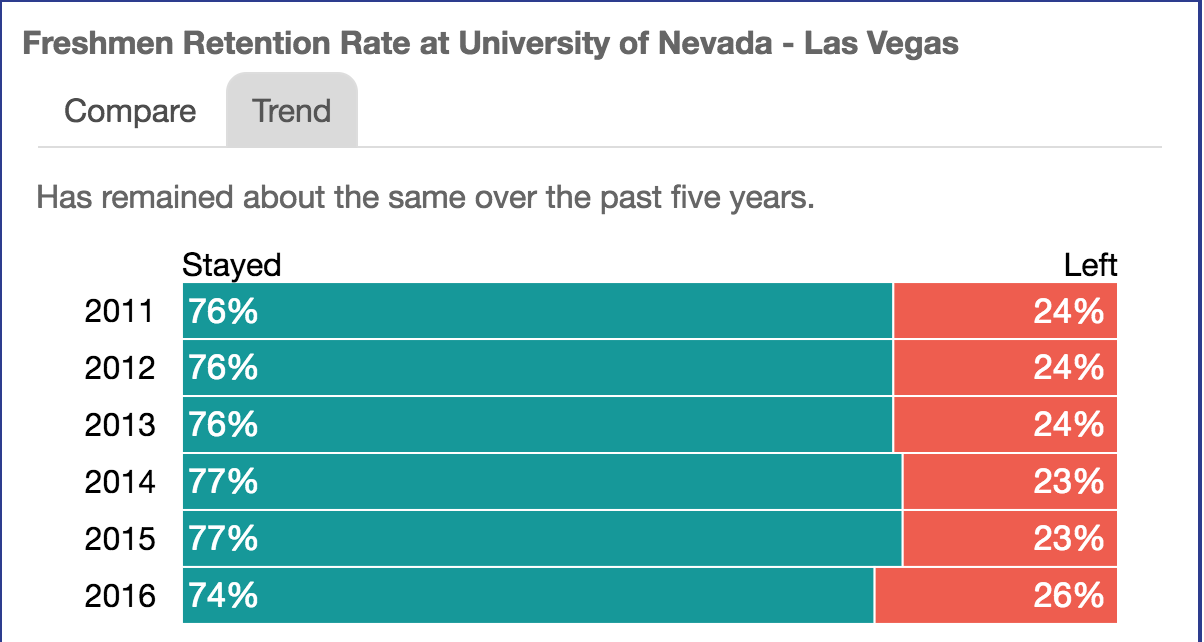
\includegraphics[scale=0.7]{unlv-retentiontrend}
	\caption{Freshmen Retention Rates at UNLV}
	\label{fig:unlv_retention_trend}
\end{figure}

\section{Objective}\label{section:objective}
The objective of this thesis is to create predictive models that can be used to identify at-risk students. In this thesis, important machine learning algorithms such as Logistic Regression, Decision trees, Random Tree Classifiers and SVM's will be trained on real-time student data obtained from UNLV's enrollment census. The trained models will then be used to predict at-risk students from a test dataset which the model has not seen earlier. The models are evaluated and compared using metrics such as precision, recall, and area under the curve to determine which model provides the best results. The results of the analysis such as the evaluation metrics will be converted to risk scores which can be easily understood by the educators and administrators at UNLV. Another contribution of this thesis is to rank students based on risk scores which will be very helpful in an efficient allocation of resources as part of the intervention programs.

\section{Outline}\label{section:outline}

In Chapter \ref{chapter:introduction}, the brief topic of First-Year student retention rates, its importance to universities and the proposed approach to increase the retention rates at UNLV was described.\newline

\noindent In Chapter \ref{chapter:background}, we will discuss the existing research on improving first-year retention rates and the background information required to understand the proposed predictive approach using machine learning. It will also cover the most important and popular algorithms of machine learning.
\newline

\noindent In Chapter \ref{chapter:methodology}, we will describe the methodology adapted for the analysis. 
\newline

\noindent In Chapter \ref{chapter:experiment_results}, we will present the experimental results. The characteristics of datasets used for these methods will also be described.
\newline

\noindent In Chapter \ref{chapter:conclusion}, we will summarize the proposed methods and their results along with the possible extension of this thesis.

\chapter{Background and Preliminaries} \label{chapter:background}
\section{Related Work}\label{section:relatedwork}

The prediction of first-year student retention rates and identification of students at risk of not being retained has been a well-researched problem in the area of higher education sector for decades. Early studies involved learning the important factors that lead to student dropout by developing a theoretical model. Tinto is one of the major and earliest researchers in this area. Tinto's student engagement model \cite{tinto1999taking} has served as the basis for a large number of theoretical studies \cite{braxton2002introduction}. Similar research was carried out by Ernest Pascarella, Patrick Terenzini, and Alexander Astin, which focused more on the external factors such as the institution's administration and its policies when determining the reasons for student retention \cite{astin2012assessment}. Tinto in his 2006 study \cite{tinto2006} has stated that there has been a huge increase in the number of businesses and organizations to analyze and help institutions with the student retention problem. Later, in the same study, he revealed that there was only little change in the retention rates even with some huge businesses helping the universities. He also described the importance of external factors such as student-faculty relationships, extracurricular program, and orientation programs for first years. Moreover, he incorporated the role of academic factors into his model to make it more suitable to the college structure \cite{tinto2006}. Astin in his Input-Environment model \cite{astin2012assessment}, suggests that researchers should consider pre-college factors such as gender, race/ethnicity, family background, high school GPA  as important for student retention.

In addition to understanding the factors responsible for student dropout, the researchers were interested in identifying students at risk of not being retained in order to intervene and prevent them from dropping out. Early research included usage of statistical and analytical methods such as logistic regression and discriminant analysis for predicting student retention rates \cite{lakkaraju2015machine,marbouti2016models,adejo2017}. The results from these models showed that the learning algorithms were in fact better than many existing rule based models in learning patterns from the existing student data. Educational data mining has emerged into an important field of research in studying student retention, because of its high accuracy and robustness in working with missing data \cite{alkhasawneh2014developing}. In another study, Jay Bainbridge, James Melitski, Anne Zahradnik, Eitel J. M. Lauría, Sandeep Jayaprakash and Josh Baron used fall 2010 undergraduate students data from four different sources and applied classifiers such as logistic regression, support vector machines and c4.5 decision trees for prediction and comparison purposes\cite{bainbridge2015}. The results showed that logistic regression and SVM trees provided higher classification accuracies compared to the decision trees to predict students at risk. 

Serge Herzog a researcher from University of Nevada, Reno(UNR) campus has done some extensive research on student retention and graduate prediction. He used Decision trees and Neural networks to predict student retention of data from UNR\cite{herzog2006estimating}. FarshidMarbouti, Heidi A.Diefes-Dux, KrishnaMadhavan \cite{marbouti2016models} have compared seven different prediction models for identifying at-risk students using in-semester performance factors (i.e., grades) and based on standards-based grading.Another similar research focused on the problem of imbalanced output class distribution in the field of student retention in which the researchers tested three balancing techniques such as over-sampling, under-sampling and synthetic minority over-sampling (SMOTE) along with machine learning algorithms.

Although predictive analysis using machine learning models have proved to be very effective in identifying at-risk students, they were still not efficient and useful to educators who wanted to develop academic support programs and resources to support the identified students. The primary reason being the lack of understanding of the metrics from the predictive models by the educators. A few researchers analyzed this issue at the high school level and came up with a framework to convert model accuracies to risk scores that could be used by the educators in the efficient allocation of the resources \cite{lakkaraju2015machine}. Though the above-mentioned framework was giving good results, it was restricted to school level data and thus cannot yield accurate results in the university level as both are very different environments with different set of factors. Hence, in this thesis we try to include such an analysis into college level studies of UNLV and compare our results to the existing approaches.


\section{Preliminaries}\label{section:preliminaries}

\subsection{Machine Learning Concepts}

\noindent  Tom Mitchell defined Machine Learning as \cite{Mitchell1997}: 
\newline\newline
\hangindent=0.7cm "A computer is said to learn from experience E with respect to some class of tasks T and performance measure P, if its performance at tasks in T, as measured by P, improves with experience E." \newline 

\noindent Example: playing chess.

\noindent E = the experience of playing many games of chess with different people

\noindent T = the task of playing chess.

\noindent P = the probability that the program will win the next game.\newline 

\noindent In general machine learning tries to learn patterns inherent in the underlying data and remembers it as experience, which it uses for predictions. It was conceptualized from the notion of learning process adopted by a human brain. Just as the human brain gets better at a specific task by repeated learning and previous experiences, a computer will also learn more patterns hidden in the data based on its previous experiences. Additionally the huge processing power of computers enables them to perform such a learning process in identifying patterns from complex data which can be very difficult for a human to understand.

\subsection{Predictive Analytics}
Predictive analytics primarily deals with extracting patterns using machine learning models from existing datasets. the extracted patterns are used to predict future events and behaviors in previously unseen data. Predictive analytics is being used in wide range of fields such as education, finance, automobile, and healthcare. The analytics is performed by running different machine learning algorithms on previously collected data. The algorithms try to learn patterns between different properties of the data and preserve the knowledge in model parameters. The resulting model is able to predict the unknown property of a future unseen data.

 \begin{table}[!t]
	\renewcommand{\arraystretch}{1.3}
	\caption{Admissions data at a University}
	\label{table:example_db}
	\centering
	\begin{tabular}{|c|c|c|c|c|}
		\hline
		\bfseries Age & \bfseries Gender & \bfseries HSGPA & \bfseries ACT & \bfseries Accepted\\
		\hline
		$20$ & Male & 3.89 & 25.6 & 1\\ \hline
		$21$ & Female & 3.20 & 22.6 & 1\\ \hline
		$20$ & Female & 2.50 & 18.3 & 0\\ \hline
		$22$ & Male & 3.10 &  19.2 & 0\\ \hline
		$19$ & Female & 3.60 & 23.5 & 1\\ \hline
	\end{tabular}
\end{table}



An illustrative example is shown in Table \ref{table:example_db} which shows student data captured during admissions at a university. The aim is to predict if the student will be accepted or not by looking at the other variables in the data. The column "Accepted" is said to be a dependent variable, and all the other variables are called independent variables. A "1" in the "Accepted" column represents the outcome of the student being accepted into the university and a "0" means he was rejected. To this data we apply a machine learning algorithm, that will learn a prediction model based on the relations between the input independent variables and the output dependent variable. The learned model is then able to predict the output variable by taking other variables as input.
  \begin{figure}
	\centering
	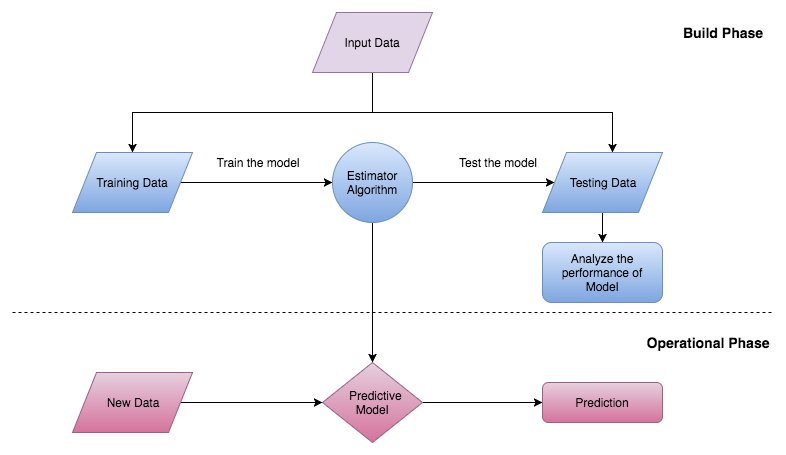
\includegraphics[scale=0.5]{MLApproachFinal}
	\caption{Machine Learning Approach}
	\label{fig:predictive_analysis-approach}
\end{figure}
 

The general approach for applying predictive analysis on a data can be divided into 2 phases as shown in figure \ref{fig:predictive_analysis-approach}. Build phase deals with the process of creating a prediction model and testing its performance. The process of creating the prediction model is known as training and the data used is known as training data. To test the effectiveness of the created model, it is tested on another set of previously unseen data known as testing data. We use two different data sets to check the generalization capacity of the model in predicting previously unseen data. If we use all the available data for training, the model may learn too much from the inputs giving rise to the problem of overfitting. Overfitting occurs when a model is performing well on its training data, but not on the other unseen data. A common approach to handle the problem of overfitting is to divide the input data into training and testing sets. The model is then evaluated for performance using test data.  The evaluated model is used in the operational phase to perform predictions given a new data. The metrics used to evaluate a model are explained in detail in coming chapters.


\subsection{Selected Models}

In this section we discuss various models that were used in this thesis to analyze the student data from UNLV. The models selected for comparison were Logistic Regression, Decision Trees, Random Forest, and SVM's.

\subsubsection {Logistic Regression Model}

Logistic Regression is a Machine Learning classification algorithm that is used to predict the probability of a categorical dependent variable. In logistic regression, the dependent variable is a binary variable that contains data coded as 1 (yes, success, etc.) or 0 (no, failure, etc.). In other words, the logistic regression model predicts P(Y=1) as a function of X.

\subsubsection {Decision Trees}

\subsubsection {Random Forest Classifiers}

\subsubsection {Support Vector Machines }

\subsection {Evaluation Methods}

\chapter{Methodology} \label{chapter:methodology}

\section{Data Collection}

The Operations Support and Reporting Office at UNLV is responsible for extracting information regarding student enrollment and performance from the UNLV Data Warehouse and reporting the census to Integrated Postsecondary Education Data System (IPEDS). The data used in this thesis were obtained from the census data submitted to IPEDS every year. The following subsections will describe more information about the data.

\section {Data Preparation}
\subsection{Data Description}
The census data from the Operations Support and Reporting Office was exported into a .csv file to be used by the analysis. The raw data consisted of a total of 17,709 freshmen student records captured cohort-wise from the academic year 2012 to 2016. The data consisted of a variety of information about each student, such as pre-college academics, standardized test scores, the social and economic status of the student, freshmen year academics and finally if the student was retained in the sophomore year. Additionally, the data had variables which were not related to the first year student retention rates. After some research and insights from experts of the domain, the raw data was cleaned to only include data that would be associated with the analysis. The following subsections describe in detail about the dataset. 
 
\subsection{Feature Extraction}
Feature extraction involves creating important useful features from the available raw data. Based on the problem statement and the data collection techniques at UNLV. The raw data was used to generate the following important features.

\subsubsection {Computation of SAT\_ACT\_Score Variable}
The admissions office at UNLV requires the students to report scores of standardized exams such as ACT and SAT during their admission process. From the raw dataset, we noticed that the ACT and SAT scores were missing for many students. Especially 56\% of students did not have ACT scores while only 28\% did not have SAT scores. Hence to capture the importance of the standardized scores into our analysis, we converted the available ACT composite scores to equivalent 
SAT composite scores based on the conversion table from \cite{ACTSAT}. The term SAT\_ACT\_Score was used to refer to this converted scores variable.

\subsubsection {Computation of F2\_Not\_Retained Variable}
The main focus of this thesis is to identify the students who are at the risk of not being retained after their freshmen year. In the raw dataset the flag F2\_Retain captures the aspect of student being retained and hence can serve as the outcome variable. We then compute the complement of this flag to obtain the feature F2\_Not\_Retained which takes 0 if the student was retained and 1 if the student was not retained. The problem of identifying students who are at the risk of not being retained after first year is then a binary classification task with F2\_Not\_Retained as the outcome variable.

\section {Data Preprocessing}
Data Preprocessing is a technique that is used to convert the raw data into a clean data set. In other words, whenever the data is gathered from different sources it is collected in raw format which is not feasible for the analysis.
Therefore, certain steps are executed to convert the data into a tiny clean dataset. This technique is performed before the execution of any predictive Analysis. 


\subsection {Handling Outliers in Data}

Generally the process of collecting data from different sources can introduce outliers into the dataset. This may be due to a faulty data extraction program or a human error. In predictive data analysis outliers can have significant effect on the predictive power of the models as they can introduce huge bias into the model. Hence it is almost always essential to check for outliers in the dataset before performing any analysis. Outliers were identified in our dataset. Data plots with index on x-axis and values on y-axis was used to demonstrate the presence of outlier in a feature.


\subsubsection{UnwHSGPA scores}

\begin{figure}
\centering
    \begin{subfigure}[b]{0.55\textwidth}            
            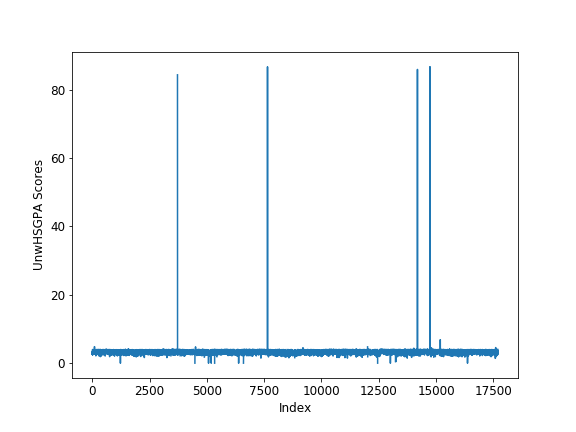
\includegraphics[width=\textwidth]{UnwHSGPAScores}
            \caption{UnwHSGPA with Outliers}
            \label{fig:UnwHSGPA-with-outliers}
    \end{subfigure}%
     %add desired spacing between images, e. g. ~, \quad, \qquad etc.
      %(or a blank line to force the subfigure onto a new line)
    \begin{subfigure}[b]{0.55\textwidth}
            \centering
            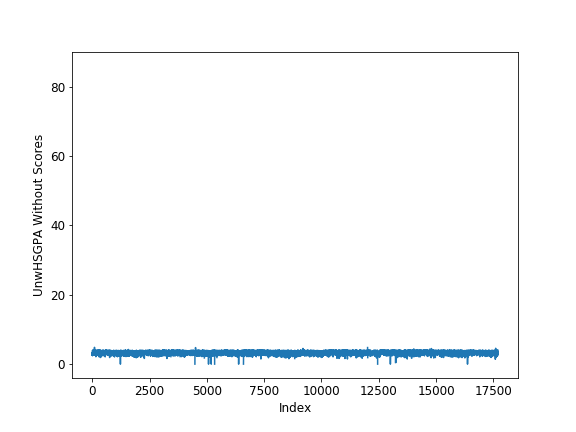
\includegraphics[width=\textwidth]{UnwHSGPAWithoutScores}
            \caption{UnwHSGPA without Outliers}
            \label{fig:UnwHSGPA-No-outliers}
    \end{subfigure}
    \caption{Removing Outliers from UnwHSGPA}\label{fig:unwHSGPA}
\end{figure}

 There were a few outliers identified for variable UnwHSGPA, as shown in figure \ref{fig:UnwHSGPA-with-outliers}. The outliers of the UnwHSGPA were replaced by mean value of the said dataset excluding all the outliers. Data plot of the variable UnwHSGPA after removing outliers is shown in figure \ref{fig:UnwHSGPA-No-outliers}


\subsection {Handling Missing Values}
In this subsection we will discuss how we handled missing values in the dataset. The table \ref{table:missing_db} shows variables along with the count of missing values. Machine learning deals with the usage of mathematical models on the data and hence it cannot be applied to datasets that have missing values. The general approach is to fill the missing value with a suitable value. The process of filling missing values in the data is known as Imputation. Researchers frequently use the mean, mode or median of the observed given values to substitute in the missing field.
 \begin{table}[!t]
	\renewcommand{\arraystretch}{1.3}
	\caption{Variables with missing values and their count}
	\label{table:missing_db}
	\centering
	\begin{tabular}{|c|c|}
		\hline
		\bfseries Variable & \bfseries Number of missing values \\
		\hline
		SAT\_ACT\_Score & 830\\ \hline
		UnwHSGPA & 1933\\ \hline
		CoreHSGPA & 3463\\ \hline
		F1\_MidtermGPA & 286\\ \hline
		F1\_MathGradePass & 4989\\ \hline
	\end{tabular}
\end{table}

\subsubsection {Imputing SAT\_ACT\_Score}
The SAT\_ACT\_Score variable had 830 missing values. By looking at the table, it can be inferred that presence of missing values in SAT\_ACT\_Score variable had very little impact on the percentage of students not being retained. A total of 24.1\% students were not retained when a value was present in the variable and 25.6\% were not retained when the variable had a missing value.

\begin{figure}[!htbp]
	\centering
	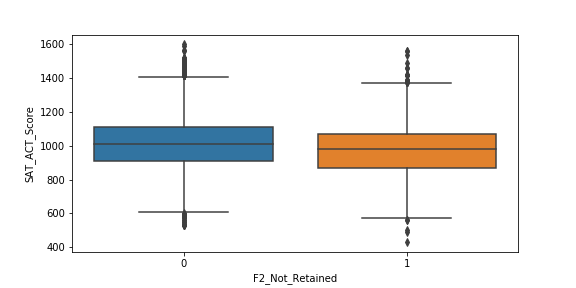
\includegraphics[scale=0.7]{SATBoxPlot}
	\caption{Boxplot of the SAT\_ACT\_Score vs F2\_NotRetained}
	\label{fig:Sat_F2NotRetained_plot}
\end{figure}

Moreover, the boxplot of the SAT\_ACT\_Score vs F2\_NotRetained (Figure \ref{fig:Sat_F2NotRetained_plot}) also shows that SAT\_ACT\_Score has very low impact on the student dropout. Based on the above facts, the missing values in this variable were replaced by the mean value. 

\subsubsection {Imputing CoreHSGPA and UnwHSGPA}
The CoreHSGPA variable had 3463 missing values, whereas the UnwHSGPA had 1943 missing values. Before imputing, we tried to analyze the relation between both the variables (Figure \ref{fig:diffHSGPA}). For this we calculated the difference between CoreHSGPA and UnwHSGPA of available records and plotted them as shown in figure \ref{fig:Core_Unw_diff}. We can clearly observe that majority of the differences were lying in the range of [-1,1], which indicates that the two variables had very close relation. Similar pattern was revealed from the distribution plot of the variable differences as shown in figure( \ref{fig:Core_Unw_dist}), which revealed that the differences followed a gaussian distribution with a mean of 0.23. Based on the above facts, we replaced the missing values with the available variable scores. The remaining missing values were replaced by the mean value of the respective variable.


\begin{figure}[!htbp]
\centering
    \begin{subfigure}[b]{0.55\textwidth}            
            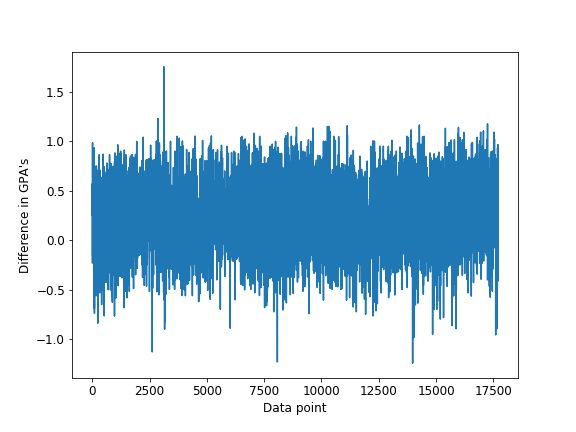
\includegraphics[width=\textwidth]{Core-Unw-GPA-diff}
            \caption{Difference between CoreHSGPA and UnwHSGPA}
            \label{fig:Core_Unw_diff}
    \end{subfigure}%
     %add desired spacing between images, e. g. ~, \quad, \qquad etc.
      %(or a blank line to force the subfigure onto a new line)
    \begin{subfigure}[b]{0.55\textwidth}
            \centering
            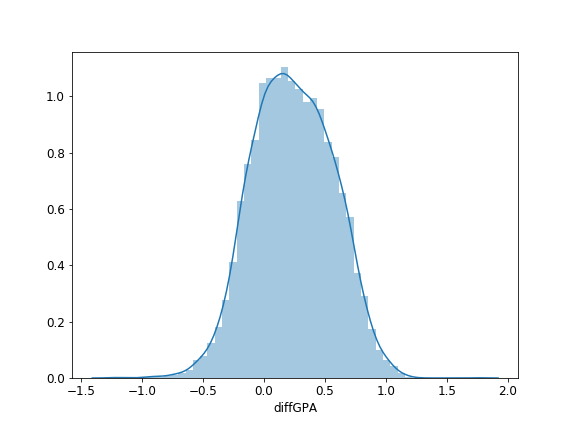
\includegraphics[width=\textwidth]{Core-Unw-GPA-distribution}
            \caption{Distribution }
            \label{fig:Core_Unw_dist}
    \end{subfigure}
    \caption{Analyzing difference between CoreHSGPA and UnwHSGPA }\label{fig:diffHSGPA}
\end{figure}

\subsubsection {Imputing F1\_MidtermGPA}

\begin{figure}[!ht]
	\centering
	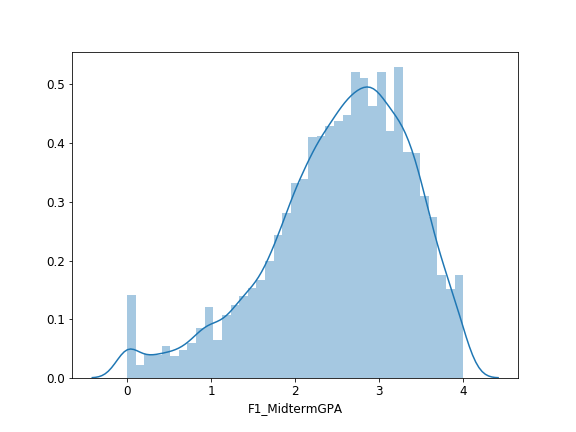
\includegraphics[scale=0.7]{F1-MidTermGPA-distribution}
	\caption{Distribution plot of the F1\_MidtermGPA}
	\label{fig:F1_MidtermGPA_plot}
\end{figure}

The F1\_MidtermGPA variable had 286 missing values which adds up to a very small percentage in the overall data. We analyzed the distribution plot of F1\_MidtermGPA (figure \ref{fig:F1_MidtermGPA_plot}) and noticed that it also follows a gaussian distribution with mean value of 2.5272 and a standard deviation of 0.851. Considering the above information we imputed the missing value of the variable with its mean as it would not shift the centrality of the variable.

\subsubsection {Imputing F1\_MathGradePass}
F1\_MathGradePass is a categorical variable with values 'Y' or 'N', where a 'Y' represents if a student got a passing grade in math taken during his first fall term and 'N' if he got a failing grade. It had a total of 4989 missing values in the variable. Such a large number of missing values for this variable is attributed to the fact that a student who did not take any math course will not have a value in this variable. Hence the missing value was replaced with a 'N'.


\subsection {Data Selection and Transformations}
What important data did you select for your analysis
\subsection {Correlation of Features}
check the correlation of factors

\section{Exploratory Data Analysis}
Exploratory data analysis (EDA) is an approach employed to analyze data sets and summarize their main characteristics, often with visual methods, without making any assumptions about its contents. It is a crucial step to take before diving into machine learning or statistical modeling because it provides the context needed to develop an appropriate model for the problem at hand and to correctly interpret its results. In this section we try to uncover some important patterns inherent in our data with appropriate plots.

\subsection {Academic years Vs F2\_Not\_Retained}
As a first step, the proportion of students retained and not retained in an academic year was plotted in the figure \ref{fig:AcadYear_F2NotRetained_plot}, to understand the distribution of students dropping out at the end of each year. Each cohort includes data about students who were in their F1 semester in that specific year. From the plot, we can infer that the number of students who drop out after their first-year varies  very slightly for each year. This observation informs us that the retention rates at UNLV are almost similar even though efforts are being made to improve them.

\begin{figure}[!htbp]
	\centering
	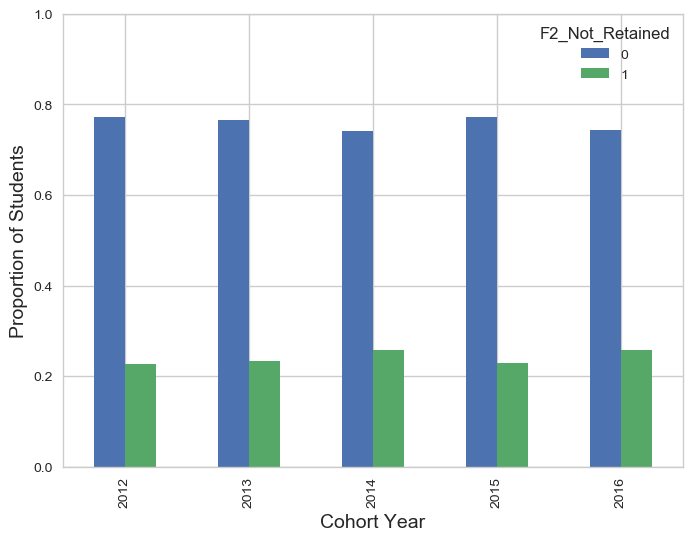
\includegraphics[scale=0.6]{NotRetained_fre_acadyear}
	\caption{Academic Year vs F2\_NotRetained}
	\label{fig:AcadYear_F2NotRetained_plot}
\end{figure}

\subsection {IPEDS Race Vs F2\_Not\_Retained}
In this section, we tried to analyze the patterns observed by different categories of the IPEDS Race with respect to student retention. For this, we plotted the different IPEDS Race categories on x-axis and the number of students who retained and who did not on y-axis as shown in figure \ref{fig:ipeds_F2NotRetained_plot}. We observed that the student population of different races was very different at UNLV with higher populations of Asian, Hispanic and White. Moreover, we also observe that the number of students retained in each race category varies quite distinctively owing to the differences in the population, however we observe that the Asian category has the best retention rates followed by Hispanic and White categories. On the whole, the figure clearly displays that the student's race is useful in predicting if he/she will be retained after the first year.

\begin{figure}[!ht]
	\centering
	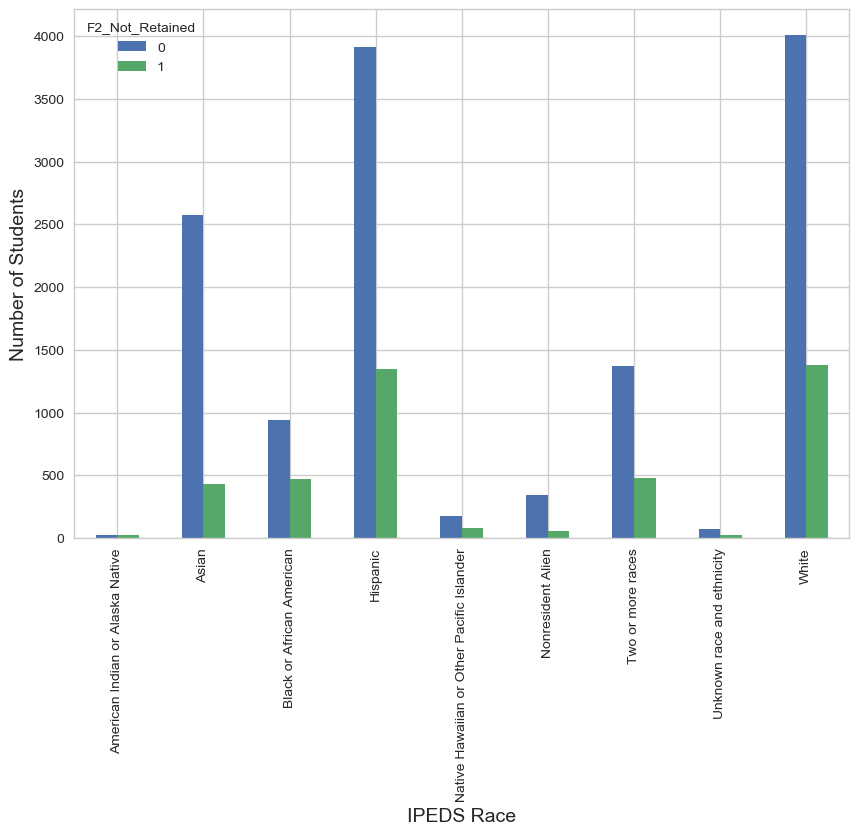
\includegraphics[scale=0.65]{ipeds_vs_notretained_stack}
	\caption{IPEDS Race vs F2\_NotRetained}
	\label{fig:ipeds_F2NotRetained_plot}
\end{figure}

\subsection {Mom\_Education\_Level Vs F2\_Not\_Retained}
In this section, we tried to analyze the patterns observed by different categories of the Mom's Education Level with respect to not retention after first year. For this, we plotted the different categories of Mom\_Education\_Level variable on x-axis and the proportion of students who retained and who did not on y-axis as shown in figure \ref{fig:mom_edu_F2NotRetained_plot}. We observed that the proportion of students who were not retained was different for different categories. We noticed that the Asian race had lowest proportion, whereas American Indian or Alaska Native had highest proportion of student dropout. On the whole, the figure clearly displays that the student's race is useful in predicting if he/she will be retained after the first year.

\begin{figure}[!ht]
	\centering
	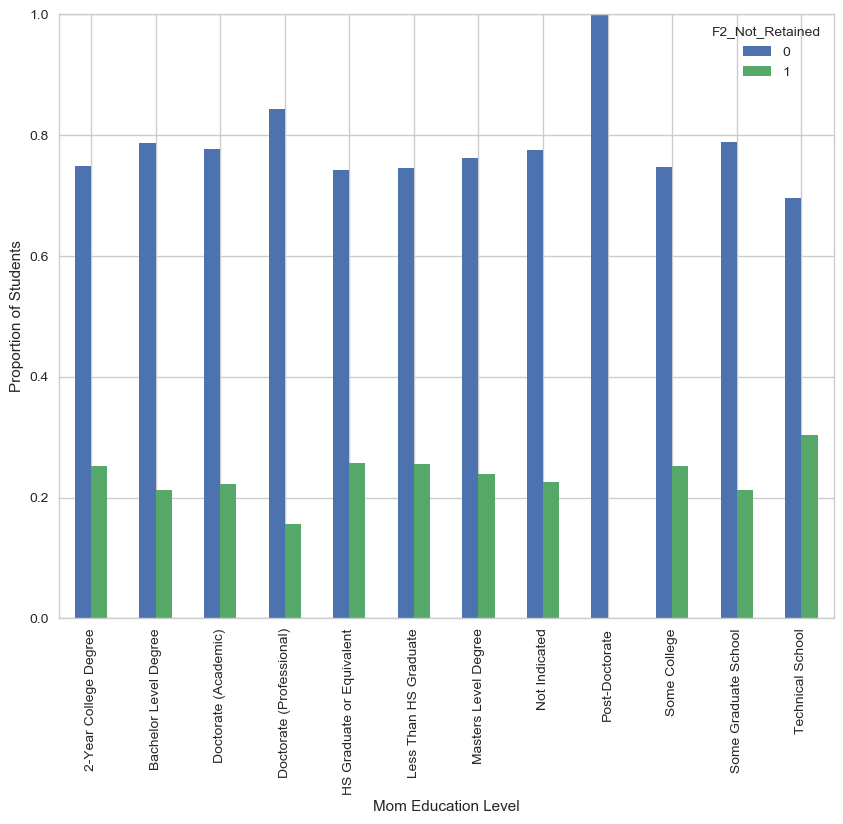
\includegraphics[scale=0.65]{NotRetained_fre_mom_edu}
	\caption{Mom's Education Level vs F2\_NotRetained}
	\label{fig:mom_edu_F2NotRetained_plot}
\end{figure}

Explain about the plots for each academic years.
Explain about ipeds race and not retained
Explain about mom and dad's education level and its influence on students retention

find out more about GPA's, SAT and their dependence on not retained.

\chapter{Experimental Results} \label{chapter:experiment_results}
\section {Analysis of Predictive Models}
\subsection {Evaluation using Traditional Metrics}
\chapter{Conclusion} \label{chapter:conclusion}
%%%
%%% The bibliography - you can change the alpha to suit your style if you don't like it is it is.
%%% The bib file should be called 'thesis.bib' - if not then change the second line here to be correct.
\bibliographystyle{alpha}
\thesisbibliography{thesis}


%%%
%%% Vita comes next
\vita
\chapter{} %% please leave this one blank - the vita stuff is sort of a hack.
\linespread{1.3} 
\begin{center}
Graduate College\\
University of Nevada, Las Vegas\\[1cm]
Aditya Rajuladevi\\[1cm]
\end{center}

\noindent Degrees:\\
\indent Bachelor Degree in Computer Engineering 2014\\
\indent Jawaharlal Nehru Technological University, Hyderabad, India\\

\noindent Thesis Title: A Machine Learning Approach to Predict First-Year Student Retention Rates at University of Nevada, Las Vegas\\

\noindent Thesis Examination Committee:\\
\indent Chairperson, Dr. Fatma Nasoz, Ph.D.\\
\indent Committee Member, Dr. Laxmi Gewali, Ph.D.\\
\indent Committee Member, Dr. Justin Zhan, Ph.D.\\
\indent Graduate Faculty Representative, Dr. Magdalena Martinez, Ph.D.\\

\end{document}





